\hypertarget{interface_t_p_chart_line}{
\section{TPChartLine Class Reference}
\label{interface_t_p_chart_line}\index{TPChartLine@{TPChartLine}}
}
{\tt \#import $<$TPChartLine.h$>$}

Inheritance diagram for TPChartLine::\begin{figure}[H]
\begin{center}
\leavevmode
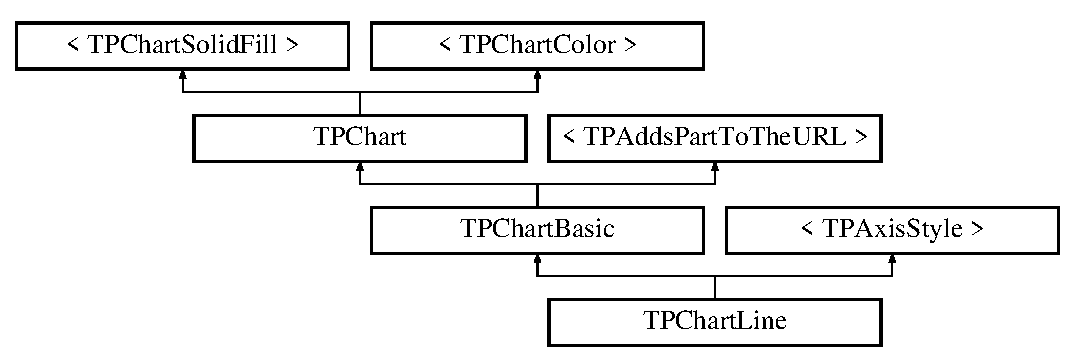
\includegraphics[height=3.31361cm]{interface_t_p_chart_line}
\end{center}
\end{figure}
\subsection*{Public Member Functions}
\begin{CompactItemize}
\item 
(NSURLRequest $\ast$) - \hyperlink{interface_t_p_chart_line_2fa4ce27ed67bce0c2d0d2a9b41c026c}{imageRequest}
\end{CompactItemize}
\subsection*{Properties}
\begin{CompactItemize}
\item 
TPChartTypeLine \hyperlink{interface_t_p_chart_line_04e85b606d425d8329ea5f9b0ec0f50f}{type}
\end{CompactItemize}


\subsection{Detailed Description}
Line chart example \href{http://chart.apis.google.com/chart?chs=200x125&cht=ls&chco=0077CC&chd=t:27,25,60,31,25,39,25,31,26,28,80,28,27,31,27,29,26,35,70,25}{\tt http://chart.apis.google.com/chart?chs=200x125\&cht=ls\&chco=0077CC\&chd=t:27,25,60,31,25,39,25,31,26,28,80,28,27,31,27,29,26,35,70,25} 

\subsection{Member Function Documentation}
\hypertarget{interface_t_p_chart_line_2fa4ce27ed67bce0c2d0d2a9b41c026c}{
\index{TPChartLine@{TPChartLine}!imageRequest@{imageRequest}}
\index{imageRequest@{imageRequest}!TPChartLine@{TPChartLine}}
\subsubsection[{imageRequest}]{\setlength{\rightskip}{0pt plus 5cm}- (NSURLRequest $\ast$) imageRequest }}
\label{interface_t_p_chart_line_2fa4ce27ed67bce0c2d0d2a9b41c026c}


inherited from superclass 

Reimplemented from \hyperlink{interface_t_p_chart_34d673557c84b693e02cd5fe587b9c6f}{TPChart}.

\subsection{Property Documentation}
\hypertarget{interface_t_p_chart_line_04e85b606d425d8329ea5f9b0ec0f50f}{
\index{TPChartLine@{TPChartLine}!type@{type}}
\index{type@{type}!TPChartLine@{TPChartLine}}
\subsubsection[{type}]{\setlength{\rightskip}{0pt plus 5cm}- (TPChartTypeLine) type\hspace{0.3cm}{\tt  \mbox{[}read, write, assign\mbox{]}}}}
\label{interface_t_p_chart_line_04e85b606d425d8329ea5f9b0ec0f50f}


type of the chart one of the following: TPChartTypeLineC, TPChartTypeLineS or TPChartTypeLineXY 

The documentation for this class was generated from the following files:\begin{CompactItemize}
\item 
TPChartLine.h\item 
TPChartLine.m\end{CompactItemize}
